% file: tournament_4_rep_6_1.tex
% created by Orbiter tikz interface
% creation date: Sat Jul 30 08:28:14 +03 2022
% DeviceCoordinates 0 0 1000000 1000000
% UserCoordinates 0 0 10000 10000
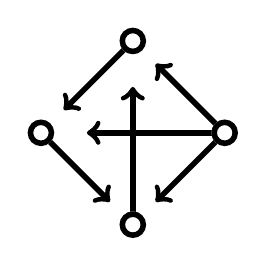
\begin{tikzpicture}[scale=0.1,line width = 2pt]
\draw [->] (28.3333,16.6667) -- (19.5833,25.4167);
\draw [->] (28.3333,16.6667) -- (10.8333,16.6667);
\draw [->] (28.3333,16.6667) -- (19.5833,7.91667);
\draw [->] (16.6667,28.3333) -- (7.91667,19.5833);
\draw [->] (16.6667,5) -- (16.6667,22.5);
\draw [->] (5,16.6667) -- (13.75,7.91667);
\filldraw[color=white] (28.3333,16.6667) circle [radius = 1.33333cm];
\draw (28.3333,16.6667) circle [radius = 1.33333cm];
\filldraw[color=white] (16.6667,28.3333) circle [radius = 1.33333cm];
\draw (16.6667,28.3333) circle [radius = 1.33333cm];
\filldraw[color=white] (5,16.6667) circle [radius = 1.33333cm];
\draw (5,16.6667) circle [radius = 1.33333cm];
\filldraw[color=white] (16.6667,5) circle [radius = 1.33333cm];
\draw (16.6667,5) circle [radius = 1.33333cm];
\end{tikzpicture}
